\begin{center}\textbf{\color{red}LUYỆN TẬP}\\
	\textbf{CHUYỂN ĐỘNG THẲNG ĐỀU - CHUYỂN ĐỘNG TỔNG HỢP\\ GIA TỐC - CHUYỂN ĐỘNG THẲNG BIẾN ĐỔI ĐỀU}
\end{center}
\setcounter{ex}{0}
\Opensolutionfile{ans}[ans/BAITAPTHEMPTCD2-TN]

% ===================================================================
\begin{ex}
	An chạy bộ qua cầu vượt với vận tốc $\SI{3}{\meter/\second}$ theo hướng từ Nam đến Bắc. Đúng lúc đó Hùng chạy bộ dưới cầu vượt theo hướng từ Đông sang Tây với vận tốc $\SI{4}{\meter/\second}$. Vận tốc của An đối với Hùng là 
	\choice
	{$\SI{7}{\meter/\second}$}
	{$\SI{1}{\meter/\second}$}
	{\True $\SI{5}{\meter/\second}$}
	{$\SI{3.5}{\meter/\second}$}
	\loigiai{}
\end{ex}
% ===================================================================
\begin{ex}
	Một xe chuyển động thẳng không đổi chiều có tốc độ trung bình là $\SI{20}{\kilo\meter/\hour}$ trên  $\frac{1}{4}$ đoạn đường đầu và $\SI{40}{\kilo\meter/\hour}$ trên $\frac{3}{4}$ đoạn đường còn lại. Tốc độ trung bình của xe trên cả đoạn đường là 	
	\choice
	{$\SI{30}{\kilo\meter/\hour}$}
	{\True $\SI{32}{\kilo\meter/\hour}$}
	{$\SI{26.67}{\kilo\meter/\hour}$}
	{$\SI{35}{\kilo\meter/\hour}$}
	\loigiai{}
\end{ex}
% ===================================================================
\begin{ex}
	Khi đang chạy với tốc độ $\SI{36}{\kilo\meter/\hour}$ thì ô tô bắt đầu chạy xuống dốc. Nhưng do bị mất phanh nên ô tô chuyển động nhanh dần đều với gia tốc $\SI{0.2}{\meter/\second^2}$ xuống hết đoạn dốc có độ dài $\SI{960}{\meter}$. Thời gian ô tô chạy xuống hết đoạn dốc là 
	\choice
	{$\SI{90}{\second}$}
	{\True $\SI{60}{\second}$}
	{$\SI{160}{\second}$}
	{$\SI{20}{\second}$}
	\loigiai{}
\end{ex}
% ===================================================================
\begin{ex}
	Đồ thị độ dịch chuyển – thời gian của một vật chuyển động như hình vẽ. Vật chuyển động
	\begin{center}
		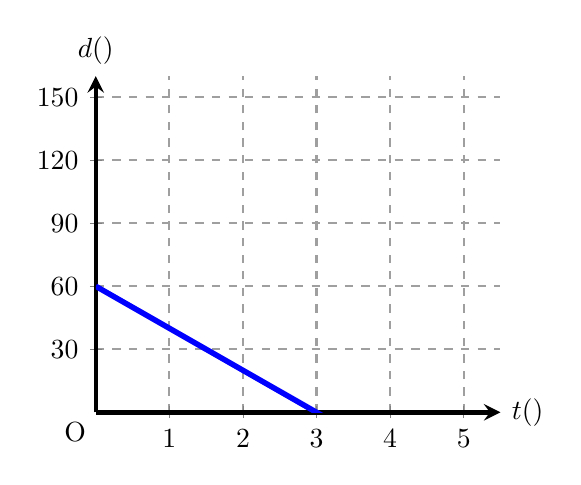
\begin{tikzpicture}  
			\begin{axis}[  ultra thick, scale=0.75,
				xmin=0,  
				xmax=5.5,  
				xtick={0,1,...,5},
				ytick={0,30,...,150},
				minor x tick num=0,
				minor y tick num=0,
				ymin=0,  
				ymax=160, 
				samples=300,
				axis lines=center, 
				grid style={step=1, line width =0.4pt, color=gray!40!white},
				grid=both, %giới hạn ô lưới
				major grid style={line width=0.8pt,gray!75!white, dashed},
				xlabel=$\xsi{t}{\left(\si{\hour}\right)}$, 		ylabel=$\xsi{d}{\left(\si{\kilo\meter}\right)}$,
				every axis y label/.style={at=(current axis.above origin),anchor=south},  
				every axis x label/.style={at=(current axis.right of origin),anchor=west},  ]
				\addplot [line width=2pt, blue, smooth, domain=0:5] {60-20*x};  
				\coordinate (O) at (axis cs: 0,0);
			\end{axis}  
			\node[below left] at (O) {O};
		\end{tikzpicture}
	\end{center}
	\choice
	{cùng chiều dương với tốc độ $\SI{60}{\kilo\meter/\hour}$}
	{\True ngược chiều dương với tốc độ $\SI{20}{\kilo\meter/\hour}$}
	{cùng chiều dương với tốc độ $\SI{20}{\kilo\meter/\hour}$}
	{ngược chiều dương với tốc độ $\SI{60}{\kilo\meter/\hour}$}
	\loigiai{}
\end{ex}
% ===================================================================
\begin{ex}
	Phương trình nào sau đây là phương trình tọa độ của một vật chuyển động thẳng chậm dần đều dọc theo trục $Ox$?
	\choice
	{$x=4-t$}
	{$x=6+t^2$}
	{$x=2-5t-t^2$}
	{\True $x=5t^2-2t+5$}
	\loigiai{}
\end{ex}

% ===================================================================
\begin{ex}
	Một vật chuyển động thẳng dọc theo trục $Ox$ có phương trình tọa độ: $x=4+20t+0,4t^2$ với $x$ tính bằng mét và $t$ tính bằng giây. Quãng đường vật đi được trong khoảng thời gian từ $t_1=\SI{1}{\second}$ đến $t_2=\SI{4}{\second}$ là
	\choice
	{$\SI{20.6}{\meter}$}
	{$\SI{26}{\meter}$}
	{\True $\SI{66}{\meter}$}
	{$\SI{67.6}{\meter}$}
	\loigiai{}
\end{ex}
% ===================================================================
\begin{ex}
	Đồ thị vận tốc - thời gian của một vật chuyển động được biểu diễn như hình vẽ. Quãng đường vật đi được từ thời điểm $t = 0$, đến thời điểm $t = \SI{60}{\second}$ là
	\begin{center}
		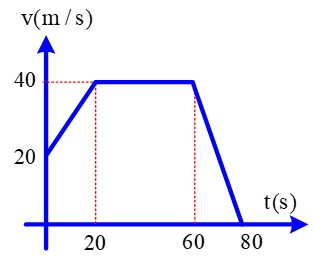
\includegraphics[width=0.3\linewidth]{figs/G10-BTTHEMPTCD-1}
	\end{center}
	\choice
	{\True $\SI{2.2}{\kilo\meter}$}
	{$\SI{1.1}{\kilo\meter}$}
	{$\SI{440}{\meter}$}
	{$\SI{1.2}{\kilo\meter}$}
	\loigiai{}
\end{ex}

% ===================================================================
\begin{ex}
	Hai xe máy cùng xuất phát từ hai địa điểm A và B cách nhau $\SI{400}{\meter}$ và cùng chạy theo hướng AB trên đoạn đường thẳng đi qua A và B. Xe máy xuất phát từ A chuyển động nhanh dần đều với gia tốc $\SI{2.5E-2}{\meter/\second^2}$. Xe máy xuất phát từ B chuyển động với gia tốc $\SI{2.0E-2}{\meter/\second^2}$. Tại vị trí hai xe đuổi kịp nhau thì tốc độ của xe xuất phát từ A và xe xuất phát từ B lần lượt là	
	\choice
	{$\SI{8}{\meter/\second}$; $\SI{10}{\meter/\second}$}
	{\True $\SI{10}{\meter/\second}$; $\SI{8}{\meter/\second}$}
	{$\SI{6}{\meter/\second}$; $\SI{4}{\meter/\second}$}
	{$\SI{4}{\meter/\second}$; $\SI{6}{\meter/\second}$}
	\loigiai{}
\end{ex}
% ===================================================================
\begin{ex}
	Lúc 8 giờ sáng một ôtô đi qua điểm A trên một đường thẳng với tốc độ $\SI{10}{\meter/\second}$, chuyển động chậm dần đều với độ lớn gia tốc $\SI{0.2}{\meter/\second^2}$. Cùng lúc đó tại điểm B cách A $\SI{390}{\meter}$, một ôtô thứ hai bắt đầu khởi hành đi ngược chiều với xe thứ nhất, chuyển động nhanh dần đều với độ lớn gia tốc $\SI{0.4}{\meter/\second^2}$. Hai xe gặp nhau ở vị trí cách A là 
	\choice
	{$\SI{240}{\meter}$}
	{\True $\SI{210}{\meter}$}
	{$\SI{250}{\meter}$}
	{$\SI{150}{\meter}$}
	\loigiai{}
\end{ex}
% ===================================================================
\begin{ex}
	Một xe máy chuyển động thẳng nhanh dần đều trên đoạn AD dài $\SI{28}{\meter}$. Sau khi xe qua A được $\SI{1}{\second}$ xe tới B với vận tốc $\SI{6}{\meter/\second}$. $\SI{1}{\second}$ trước khi tới D, xe ở C với vận tốc $\SI{8}{\meter/\second}$. Thời gian xe đi trên đoạn đường AD là
	\choice
	{$\SI{10}{\second}$}
	{$\SI{7}{\second}$}
	{$\SI{3}{\second}$}
	{\True $\SI{4}{\second}$}
	\loigiai{
	}
\end{ex}
\Closesolutionfile{ans}
\newpage
\begin{center}
	\textbf{BẢNG ĐÁP ÁN}
\end{center}
\inputansbox{10}{ans/BAITAPTHEMPTCD2-TN}